\subsection{SoC Generation and Design Space Exploration}\label{sec:soc-generation}
As shown in Figure \ref{fig:soc-generation}, the third stage transforms the IP manifest and hardware/software partition into an executable SoC. The partition determines the coarse CPU--accelerator organization, and DSE subsequently refines the parameters of that organization using more accurate system-level feedback.

\begin{figure*}[htp]
    \centering
    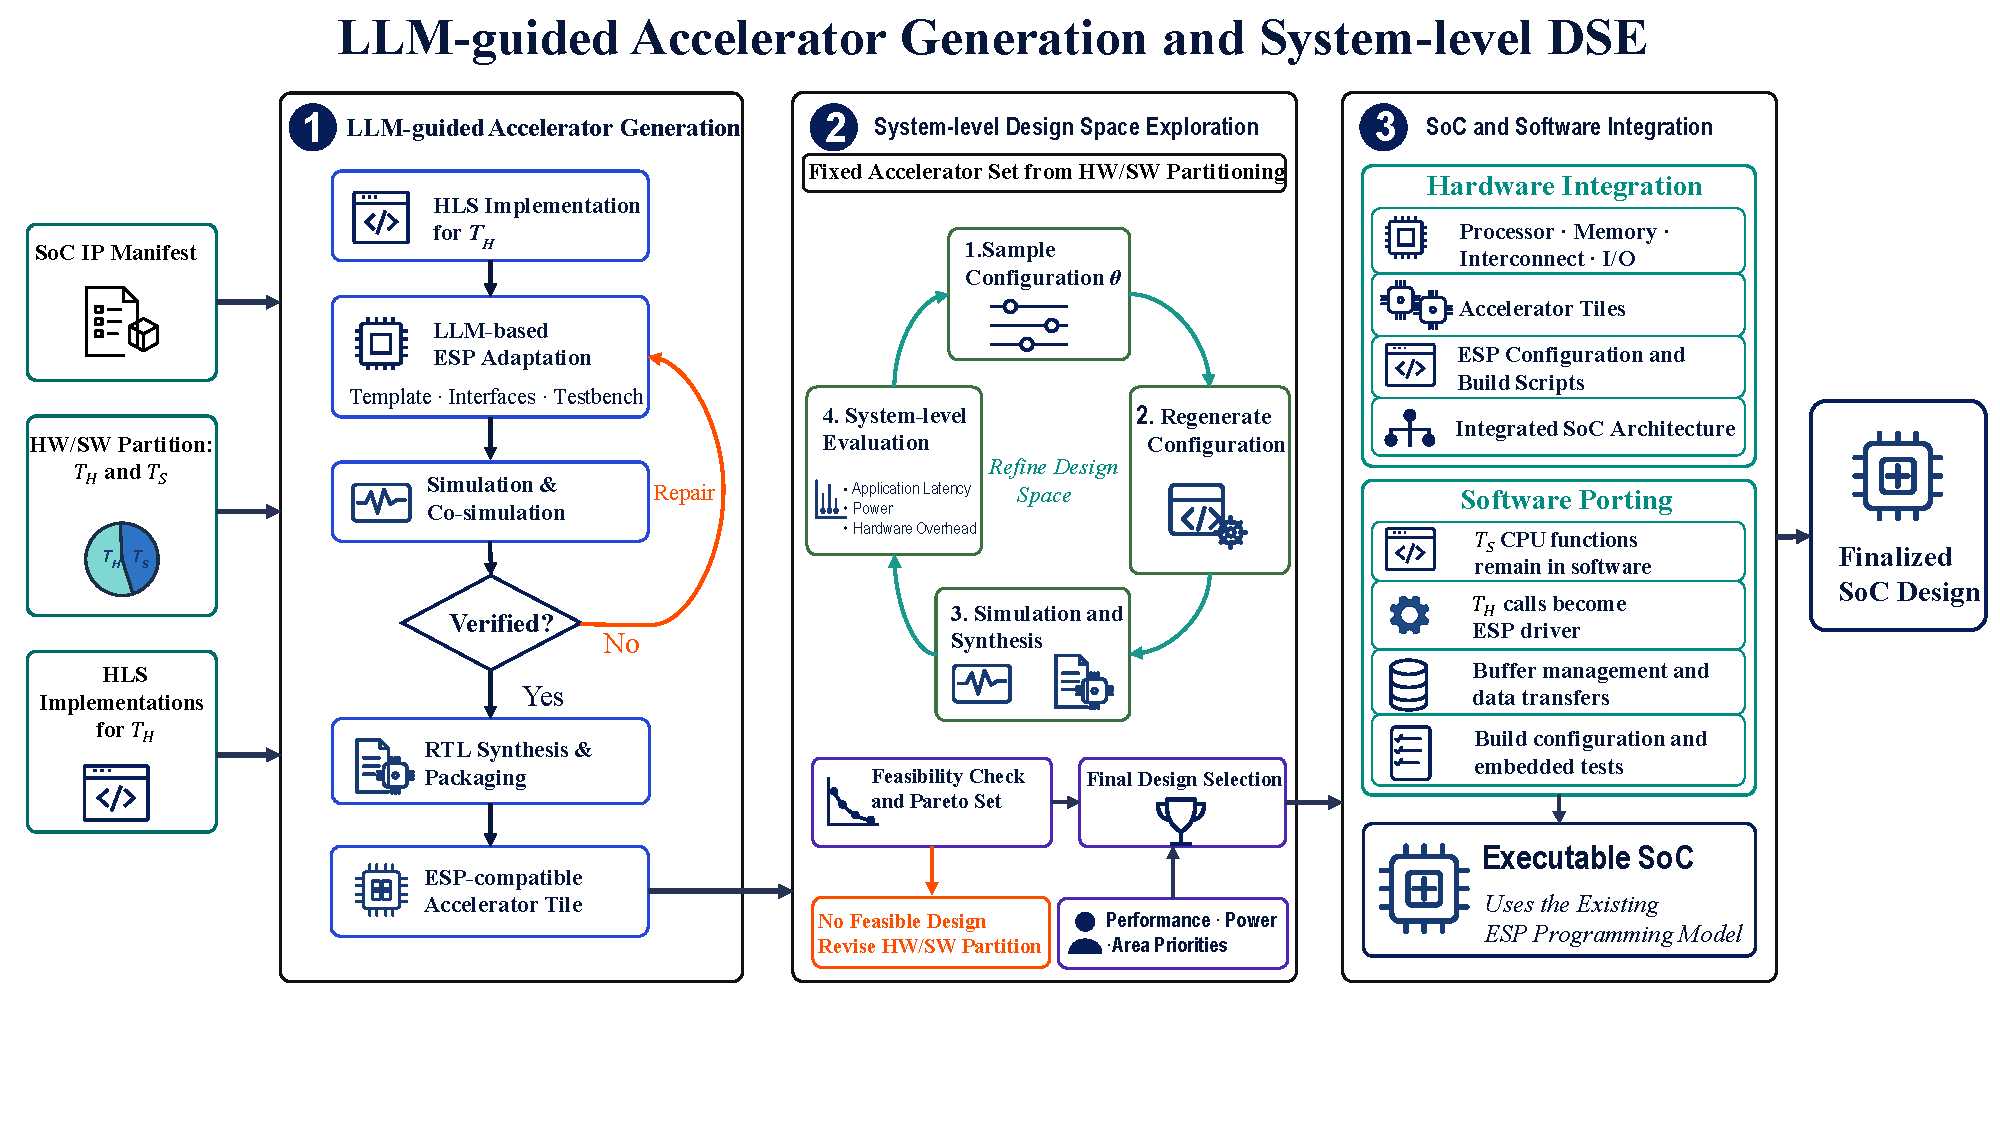
\includegraphics[width=0.92\textwidth]{pic/soc-generation.pdf}
    \caption{LLM-guided accelerator generation and system-level DSE. SoCPilot converts hardware-mapped functions into verified ESP-compatible accelerator tiles, integrates them with the selected system IPs and software, and refines the resulting SoC through system-level design space exploration. Infeasible designs trigger a revision of the hardware/software partition.}
    \label{fig:soc-generation}
\end{figure*} 


\textbf{Accelerator and SoC generation.}
SoCPilot automates the integration of HLS-generated accelerators into the ESP framework~\cite{7428012}. For each application function designated for hardware execution within $T_H$, the framework processes the synthesized hardware implementation and its interface metadata, encapsulating them into an ESP-compatible third-party accelerator. This encapsulation equips the module with the protocol adaptation, control, memory-access, and interrupt interfaces necessary for operation within the ESP architecture, while concurrently generating the requisite metadata for system-level composition. Subsequently, the packaged accelerator is registered with the ESP system-generation flow and instantiated as an accelerator tile based on the target SoC configuration. Prior to system integration, the accelerator undergoes comprehensive validation via C-level simulation, high-level synthesis, and C/RTL co-simulation, ensuring that only functionally verified hardware is incorporated into the final SoC.

Subsequently, SoCPilot constructs the target SoC by instantiating the chosen processor, memory subsystem, interconnect, I/O components, and accelerator tiles via the ESP system-configuration and generation flow. Based on the specified hardware-software partition, functions designated to $T_S$ remain processor-executed, whereas functions allocated to $T_H$ are mapped to the integrated accelerator tiles. SoCPilot generates the hardware integration scripts and build configurations required to synthesize the final SoC. The embedded application routines that configure, invoke, and communicate with the accelerators are manually implemented by the authors using ESP's established runtime API; they are neither generated nor modified by the LLM and are kept fixed during evaluation. Thus, the automated boundary of SoCPilot covers accelerator generation, packaging, SoC configuration, integration, and tool-flow orchestration, but not embedded application-code generation.

%%这需要确定dse是按照什么方式阐述
%目前是先dse生成soc之后没有进行dse
\textbf{System-level design space exploration.}
The initial partition reduces the search space by fixing which functions are implemented as accelerators. SoCPilot then explores a parameter vector $\boldsymbol{\theta}$ that covers the available processor configuration, cache hierarchy, interconnect settings, and candidate accelerator implementations produced by the HLS stage. Accelerator choices include pragma configurations and interface parameters; system choices include cache capacity and associativity, cache-line size, and NoC buffering. Table~\ref{table:node parameter-all} lists the principal dimensions used in the current implementation.
%%这个地方最终soc支持这么多但是在实际dse是仿真的dse并不支持这么多
\begin{table}[h]
     \vspace{-1em}
    \caption{Principal parameters for system-level DSE}
    \label{table:node parameter-all}
    \vspace{-0.5em}
    \resizebox{0.5\textwidth}{!}{
    \renewcommand\arraystretch{1.3}
        \begin{tabular}{cc}
        \hline
          \textbf{Design variable} & \textbf{Candidate values or source} \\ \hline
          Processor configuration & ESP-supported configurations \\
          Accelerator implementation & Pareto candidates from HLS \\
          HLS pragmas & Pipeline, unroll, and array partition \\
          Interface data width & ESP-compatible configurations \\
          Cache line size & 128, 256, 512 \\
          L2 sets & 32, 64 \\ 
          L2 ways & 2, 4, 8 \\
          LLC sets & 128, 256, 512 \\
          LLC ways & 4, 8, 16 \\
          NoC FIFO depth & 2, 4, 6 \\ \hline
        \end{tabular}} 
\end{table}

For every sampled configuration, SoCPilot regenerates the relevant ESP configuration and evaluates end-to-end latency together with the estimated area provided by the common area model. HyperMapper \cite{9124618} explores this latency--area design space: its surrogate model proposes new configurations, tool feedback updates the model, and points that violate the application-specific area constraint are discarded. The final design is selected from the feasible configurations according to the latency objective under the specified area budget. In contrast to hardware/software partitioning, this search performs fine-grained optimization around the current accelerator set. If no feasible design is found, SoCPilot returns to the previous stage and revises the hardware/software partition.

